The executed full-dimension pilot contains 3 independent seeds, with $N=500$, $p=100$, $h=252$ and 15 years per seed. These are pilot results, not the planned 500-seed final evaluation. Three separate reduced-dimension smoke seeds exercise the software only.

\begin{table}[ht]\centering\small

\begin{tabular}{lrrrr}

\toprule

Method & Utility$\times h$ & Net Sharpe & Moves & Inactive \\

\midrule

All Signals & 0.04685 & 4.078 & 0.00 & 0.000 \\

Oracle & 0.05601 & 4.915 & 0.00 & 0.000 \\

Greedy & 0.05099 & 3.951 & 9.33 & 0.071 \\

Repeated-HAC-p & 0.04335 & 3.092 & 4.00 & 0.071 \\

E-process & 0.00000 & NA & 0.00 & 1.000 \\

\bottomrule\end{tabular}

\caption{Means across executed pilot seeds. Utility is mean daily utility rescaled by $h$, not an annual certainty equivalent. Inactive paths have undefined Sharpe.}\end{table}

The public bound is $\nu^2=0.0132148$. The largest current annual log evidence is 0.006575, compared with $\log20=2.995732$. The small number of seeds is insufficient for a reliable ranking of methods. The conservative certificate and annual opportunity cost must be assessed before any assertion of economic advantage.

Separate controlled statistical diagnostics use 10,000 replications and 1600 observations. Under a predictable heteroskedastic conditional-mean-zero law, the adaptive e-process crosses at rate 0.0036 (Wilson interval [0.0026, 0.0050]). The repeated uncorrected Bartlett-HAC normal test crosses at rate 0.1894. The latter combines finite-sample approximation with repeated testing; these procedures therefore do not have matched overall type-I error. This is an individual-episode calibration experiment, not a financial-market performance result. Positive constant-mean experiments compare observed power and certificate regret with T2 bounds.

\begin{figure}[ht]\centering

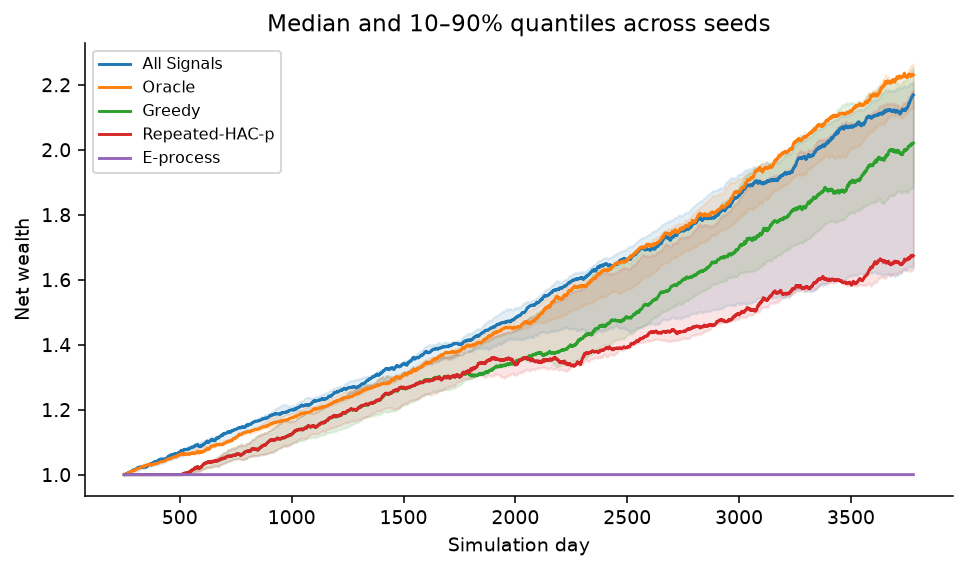
\includegraphics[width=.97\linewidth]{figures/equity_quantiles.png}

\caption{Net wealth median and 10--90 percent quantiles across the executed seeds. Each method uses identical market observations within a seed.}

\end{figure}

\begin{figure}[ht]\centering

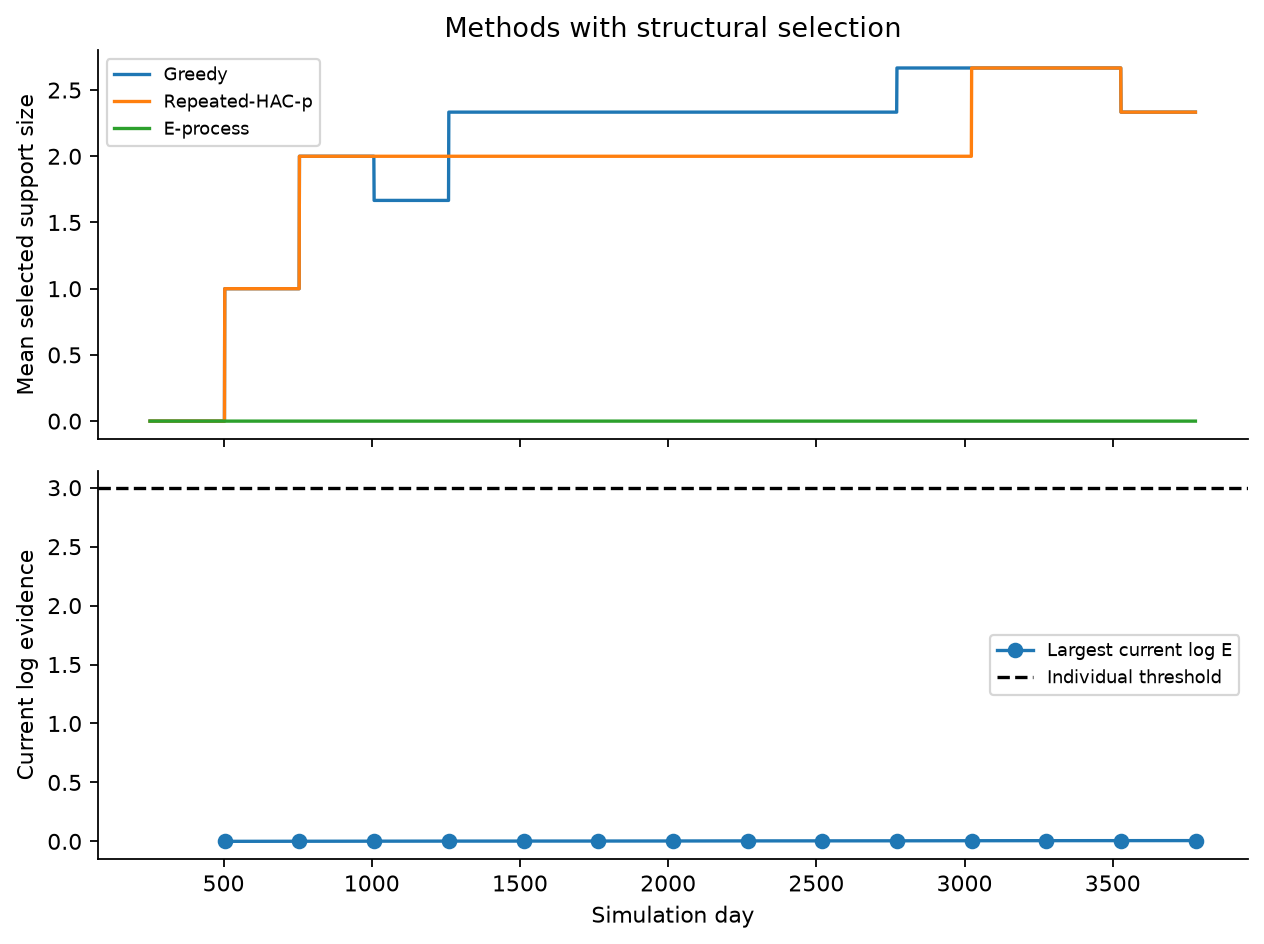
\includegraphics[width=.97\linewidth]{figures/activity_evidence.png}

\caption{Selected support size for the three search methods and largest current annual E-process evidence. All Signals and Oracle always permit all 100 signals. The threshold is individual; the search has no global 5 percent guarantee.}

\end{figure}

\begin{figure}[ht]\centering

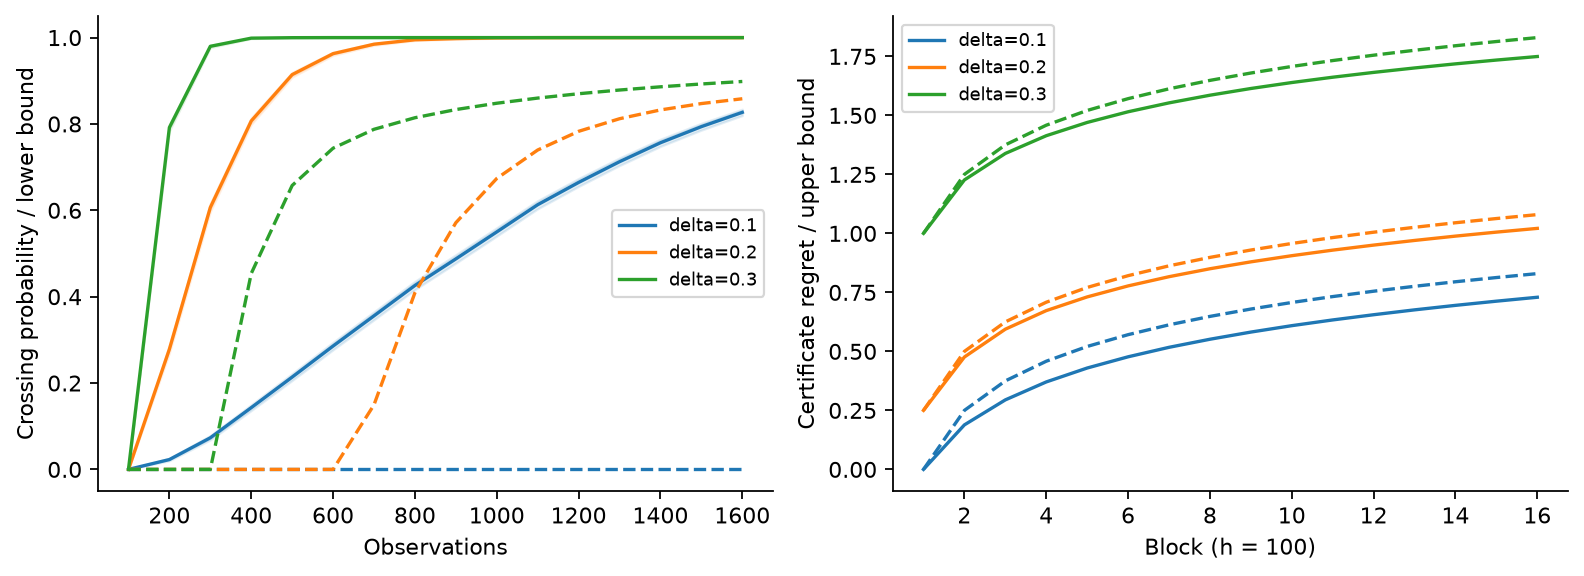
\includegraphics[width=.97\linewidth]{figures/stationary_power.png}

\caption{Controlled constant-mean statistical experiments: empirical adaptive power and certificate regret (solid), and theoretical bounds (dashed). These experiments satisfy T2 rather than the regime-changing financial model.}

\end{figure}

\clearpage
